% !TEX root = document.tex


\chapter{The Codex Metadata Format}
\label{chap:codex}

In the previous chapter,~\cref{chap:code-exploration-services}, we concluded that there exists a problem with current
systems that provide code exploration services just like there is the IDE portability problem for editor services.
We called this problem the \problem{\times} problem for code exploration services.
In this chapter we will design a prototype system we call Codex that solves this problem.
First we will more precisely define the goals of Codex, after which we will outline our approach which we will then demonstrate.

\section{The Goal of Codex}\label{sec:the-goal-of-codex}

%Codex transforms the \problem{\times} problem into a \problem{+} problem in a similar fashion to how \ac{LSP} transforms the IDE portability problem.

In an editor, source code is constantly changed, which means that any information needed for editor services must constantly be recalculated based on new changes to the source code.
With \ac{LSP}, these recalculations happen in the language-specific `language server', with which the editor must continually communicate.
Such recalculations are not always possible in other code exploration media.
To demonstrate Codex, we will focus specifically on two media in this chapter and thesis: HTML webpages and PDF documents generated through LaTeX.

Neither of these media easily support the constant recalculation we see with editor services for different reasons.

In PDF documents the reason is simple, you cannot easily execute any code in PDFs if at all.
Furthermore, when PDF documents are printed, all interactivity is certainly lost while the possibility of providing code exploration services like syntax colouring is not.
Instead, we would like to ``bake in'' the code exploration services the moment the PDF is generated by, for example colouring text, inserting hyperlinks and adding hover text.
We illustrate this in~\cref{fig:static-vs-dynamic}.

%\section{A static Language Server Protocol}\label{sec:a-static-language-server-protocol}

% Take PDF documents for example.
% Because it is near impossible to run code in PDF documents, we cannot make requests to language-specific tools like a language server.
% Instead, if we want to provide code exploration services in PDFs, we would like to essentially bake them in at the moment the PDF is generated by colouring text, inserting hyperlinks and adding hover text.

%Any information needed to provide code exploration services in a PDF is static, which means that there is no reason to request such information on-demand.
%This is true for all code exploration services: the code they provide services for does not change, by definition.

%That means that a medium with code exploration services could even bake-in the code exploration services by, for example, colouring text, inserting hyperlinks and adding hover text.

% We illustrate the difference between how an editor gathers information for editor services using \ac{LSP}, and how in \cref{fig:static-vs-dynamic}.
% In that figure, \ac{LSP} solves the
%
% We call tool that creates code presentations with baked-in code exploration services, a presentation generator, or generator for short.
% Generators are medium-specific: one generator could create PDF documents and another webpages.
% Then, to avoid the \problem{\times} problem, generators should be language agnostic and talk over a standardised interface to language-specific tools.



On Websites, interactivity is not as impossible as in PDF documents, and there are examples of web-based editors which communicate with an LSP over the internet~\autocite{che, theia}.
However, these web-editors only do that because they allow users to change code requiring constant updates.
For providing only code exploration on static webpages, the overhead is both undesired and unnecessary.
Undesired because it makes exploring code slower and unnecessary because just like with PDFs the code exploration services can be baked in to the page.

Thus goal of Codex is to show that we can support code exploration services in different media, in a language-agnostic way, while avoiding the \problem{\times} problem.
To demonstrate this two goal, we first use metadata in the Codex format to provide rich code exploration on websites and PDF documents.
Then, we show two approaches to gather metadata from code bases: adapting existing tools made to support existing languages; and to directly gathering metadata from a parser and type checker of a \ac{DSL}.
This shows how the Codex format is useful to present code for small programming languages for which no custom tooling is available.



%Although we cannot say that LSP solved the IDE portability problem, the project has considerably improved the status quo.
%Using LSP, many editors and languages can communicate.
%However, because the \ac{LSP} has a client-server architecture it is hard to
%
%To show that a metadata format can indeed power code exploration services, we have created a proof-of-concept\footnote{The source code for this proof of concept can be found on GitHub at \url{https://github.com/url-anonymized}}.
%The goal of this proof of concept is twofold:
%to demonstrate that it is feasible to use statically generated metadata to provide code exploration services in various media;
%and to show that by using a data format like ours, we can decouple the production and consumption of such static metadata in a language-agnostic way.
%
\todo{figure commented below}
\begin{figure*}[ht]
    \centering
    \begin{subfigure}[b]{0.49\textwidth}
        \centering
        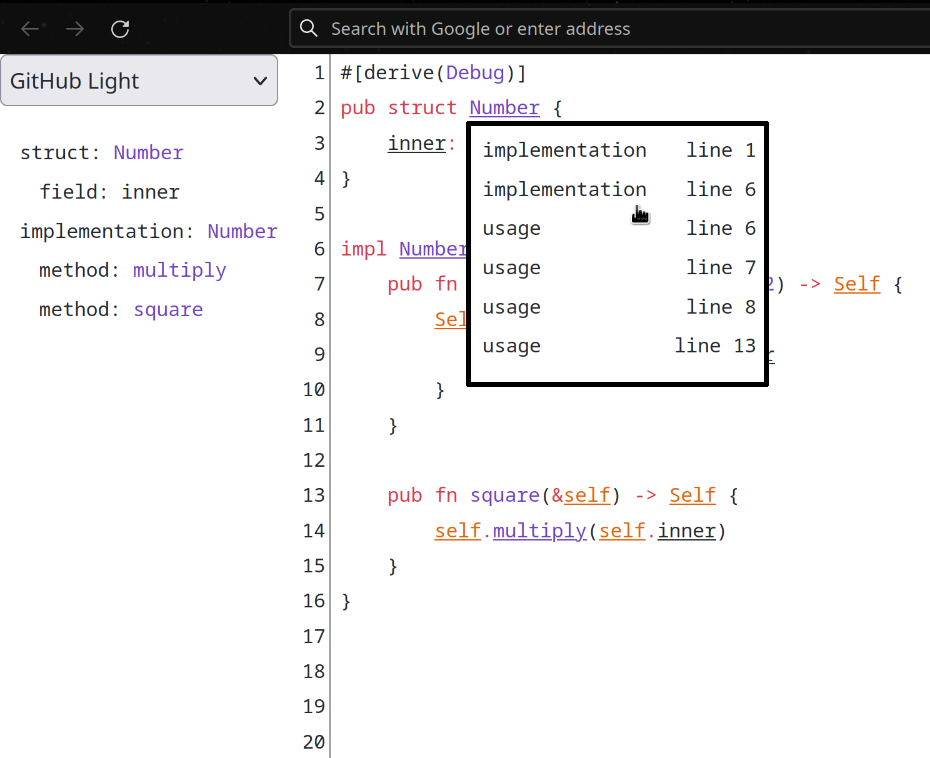
\includegraphics[width=\textwidth]{../images/codex-html}
        \caption{
            A fragment of Rust code presented in an interactive HTML webpage.
            The color information, reference information (underlines), outline, and warnings are derived from metadata stored in the Codex format.
            When a declaration in the code is referenced more than once, hovering over the underlined name opens a pop-up listing all its usages.
            Clicking one of the usages in the list instantly jumps the PDF viewer to the relevant code.
        }%
        \label{fig:demo.html}
    \end{subfigure}
    \hfill
    \begin{subfigure}[b]{0.49\textwidth}
        \centering
        \codeNumberRs
        \caption{
            The same fragment of Rust code as shown in \cref{fig:demo.html},
            but embedded in this paper through LaTeX source code generated from the Codex metadata format.
            When this paper's \acs{PDF} is viewed digitally, underlined elements are clickable and navigate to the referenced location.
            When an item is referenced more than once, superscript annotations are inserted that facilitate navigation. \\
        }%
        \label{fig:demo.latex}
    \end{subfigure}
    \caption{A demonstration of our proof of concept, presenting source code on a website and in this document.}
    \label{fig:demo}
\end{figure*}

% \paragraph{Reading this Section}
%
% In this section, we demonstrate a proof of concept of Codex.
% Part of this demonstration consists of examples of codex converting source code to LaTeX, which we display as part of this document.
% This entire section is written in a way that, when printed in black-and-white, it is readable.
% However, some parts of the demonstration will contain color, and interactive elements which will not be visible in black-and-white.
% Each example does have an explanation of what could be visible when read in color or digitally.


\section{Presenting Code on Websites through HTML}
\label{sec:demonstration.html}

HTML is a standard format for documents designed to be displayed in web browsers.
Together with CSS and JavaScript, HTML can be used to create websites with complex graphical user interfaces and visualizations.
Many websites such as StackOverflow, GitHub and GitLab can visualize users' source code, sometimes with some basic code exploration services.

In our demonstration we can produce HTML documents from source code and its corresponding Codex metadata.
A screenshot of the resulting website is shown in~\cref{fig:demo.html}.

In the generated HTML document, we implemented several code exploration services:
syntax coloring, structure outline, code navigation, and diagnostic messages.
Code navigation is implemented by adding hyperlinks to the code, though when more than one reference exists, a pop-up is shown when hovering over underlined items, allowing users to choose where to navigate.
Diagnostic messages are shown by underlining an item in yellow, which when hovered over shows the associated compiler warnings and errors.

% To generate these documents, we take the metadata, and use it to tokenize the source text.
% Tokens are spans of text which have the same metadata.
% Because the metadata is based on the syntactical structure of the code, these tokens usually correspond with syntactical elements.

% \todo[inline]{remove this}
% Then we wrap each token in HTML \texttt{span} elements, with the correct CSS classes determined based on the metadata to color each token.
% Here, we also insert link information.
% Tokens are annotated with unique identifiers that allow a JavaScript \texttt{onclick} handler to navigate the code.
% These identifiers are also used to navigate from outline items to source code.
% The outline itself is generated separately, but also uses the tokenization to highlight the pieces of code embedded in the outline.

It is possible for users to change the theme of the HTML visualization.
Instead of assigning colors to tokens, we add CSS classes based on the token's classification (See \cref{sec:demonstration.generating.textmate} for more details).
At the same time, multiple TextMate syntax theme definitions are translated to CSS and included with the HTML document.
Users can choose which CSS rules are applied by choosing a theme in the top left.


\section{Presenting Code in PDF Documents through LaTeX}
\label{sec:demonstration.latex}

A different presentation of the same Rust code of~\cref{fig:demo.html} is shown in~\cref{fig:demo.latex} embedded into this paper's text through generated LaTeX code.
Just like with HTML, the Codex proof of concept can also generate LaTeX source code based on metadata in the Codex format.
The two visualizations are adjusted to their medium, but both rely on the Codex metadata format.

% And yet, some elements are similar. Syntax is still colored (using~\texttt{xcolor}), although now with a static theme which readers cannot change.
% Underlined elements are links (using~\texttt{hyperref}), and there is a possibility to generate a digital outline in the resulting PDF document resulting from the LaTeX source.
% We have not included an outline of the code in this paper, since we think it would be distracting in this context.

One extra aspect of our LaTeX generator is that it can generate LaTeX for multiple files from the same project, if the metadata contains that information.
\Cref{fig:demo.latex.reference} shows source code from a different file in the same Rust project as the example in \cref{fig:demo}.
The two files reference each other, and when viewing this paper digitally, hyperlinks enable quick navigation between the two figures.

When there are multiple references, instead of providing a drop-down menu as shown in the generated website, in the PDF we add multiple links in superscript to parts of the code that reference multiple other locations in the code.
An example of this can found in \cref{fig:demo.latex}, \cref{fig:demo.latex.reference}, and \cref{fig:elaine}.

Because both the HTML presentation and this LaTeX presentation rely solely on metadata in the Codex format,
both are completely language-agnostic.
Although \cref{fig:codex-json-metadata} is mainly meant to demonstrate what the Codex metadata format looks like when it is serialized, the syntax coloring in the example itself is created using Codex.
Therefore, \cref{fig:codex-json-metadata} is also a demonstration of how, through the Codex metadata format, we can present code written in different languages.

% In this section, we demonstrate a proof of concept of Codex.
% Part of this demonstration consists of examples of codex converting source code to LaTeX, which we display as part of this document.
% This entire section is written in a way that, when printed in black-and-white, it is readable.
% However, some parts of the demonstration will contain color, and interactive elements which will not be visible in black-and-white.
% Each example does have an explanation of what could be visible when read in color or digitally.


\section{Generating Metadata from Existing Tools}

Codex metadata can be generated either directly by instrumenting compilers, or by adapting independently developed tools.
In this section, we show how we used several of such existing tools to generate metadata and how we converted this metadata into the Codex format.

\paragraph{TextMate Grammars}
\label{sec:demonstration.generating.textmate}

The first tool that we use to generate Codex metadata are grammar definitions.
A common standard for grammar definitions supported by code editors is the one originally used by the TextMate editor~\cite{textmate}.
Grammar definitions for many languages, both small and large, are freely available online, mostly with the purpose to be used in editors.
Almost all editors either have native support for these TextMate grammar files, or have plugins which add this support.

TextMate grammars are not full context-free grammars, but instead function by applying regular expressions to fragments of source code.
Based on which regular expressions matched words in the code, other regular expressions are brought in and out of scope to allow moderately complex syntaxes to be parsed.
Due to their design, TextMate grammars quite often perform well even in the presence of syntax errors.

TextMate introduces a way to hierarchically classify tokens based on the token's function in a programming language.
We discussed in \cref{sec:demonstration.format} how we use this function for syntax coloring and other code exploration services in the Codex format.
Because we use this system for syntax coloring, translating from TextMate output to the Codex format is very simple.
TextMate grammar files contain such classifiers, and we can put those directly into the Codex format.

% We use this hierarchical classification for syntax coloring, but also for other parts of metadata that need categorization.
% We discussed this in depth in \cref{sec:demonstration.format}, but the inspiration to use classifications in metadata came from TextMate.
% This also means that translating from a TextMate parser to the Codex format is very simple.
% TextMate grammars already contain classifications.

% \todo[inline]{Already explained}

% In Codex, TextMate grammars can be associated with a certain programming language.
% When Codex analyses a file of that programming language, and a grammar is available for that language, Codex uses the grammar to categorize the tokens in the file.

% In \cref{fig:codex-json-metadata}, we can see an example of this.
% We see that a token at offset $4$ with a length of $4$ has the syntax category \texttt{keyword.declaration.enum.rust}.
% This corresponds with the code in \cref{fig:codex-field}, where after $4$ characters, there is the keyword \texttt{enum}, which is $4$ characters long.
% The dots in this category separate hierarchical levels; after every dot, the category becomes more specific.
% Based on that category, the token is colored red in \cref{fig:codex-field} by the theme we used.

Previous parsers using TextMate (like the one for VS Code and TextMate itself) are designed to work in combination with an editor.
These proved hard to integrate in Codex, in part because they were designed to directly output color information as opposed to token classifications.
For our proof of concept, we wrote a custom TextMate parser in Rust, which we have tested on grammar definitions of many large languages such as the ones for Rust, TypeScript, and Haskell.

\paragraph{CTAGS}
CTAGS~\cite{ctags} is a tool that can provide primitive editor services in terminal-based editors such as Vim.
To do this, CTAGS parses source files of many different languages and can generate so-called tags files from that.
Vim can then read these tags files to allow programmers to search for definitions in a code base.
CTAGS does not provide enough information to derive code navigation from its output.
However, its output can be used to generate outlines for source files, which is what Codex does.
An example of such an outline can be found in \cref{fig:demo.html}.

\paragraph{The Language Server Protocol}

In \cref{subsec:language-servers}, we already mentioned \ac{LSP}~\cite{lsp} in the context of the \problem{\times} problem.
Although \ac{LSP} is a protocol mainly meant for editors, we can use the information that \ac{LSP} can provide and extract metadata from it.
This is very different from how \ac{LSP} is normally used for editor services, requiring live communication about a user's interaction with the code base.

To accomplish this, we first start a language server on the code base we analyze.
Then we query this language server about every token in a code base, storing all responses.
We then convert the responses such that they can be stored in the Codex format, after which the language server can be stopped again.
Because of the number of queries that need to be executed, this process can be rather slow, taking up a majority of the indexing time.
However, for this demonstration, speed was not a priority.

Codex currently queries \ac{LSP} to get both reference information and diagnostic messages.
However, the LSP can provide much more than just reference information, like documentation for items, code folding points and code actions.

We have tested Codex querying an \ac{LSP}, with both Rust's and Haskell's language server implementation.
This is also how the reference metadata in \cref{fig:demo.html}, \cref{fig:demo.latex} and \cref{fig:codex-field} is generated.

\todo{figure commented below}
\begin{figure}
    \centering
    \codeBRs
    \caption{This is the continuation of the example Rust code in figure \cref{fig:demo.latex}. Code navigation enables quick navigation between the two pieces of code when reading this paper digitally.}
    \label{fig:demo.latex.reference}
\end{figure}


\section{Producing Metadata for Small Languages: Elaine}
\label{sec:elaine}%
Small programming languages, \acp{DSL} or research programming languages, often have very little tooling available.
The time it costs to make tooling, such as editor services, build systems and documentation is often not worth the time.
However, for educational purposes, and science communication, having some simple code exploration services like syntax highlighting
and code navigation could be very advantageous.

The Codex format can help with this. The visualizations of code that Codex can generate are completely language-agnostic.
That means that if the compiler or interpreter of a \ac{DSL} can output metadata in the Codex format, all code exploration services in the Codex visualizations work out of the box.

% To demonstrate this, we present Elaine.
To demonstrate this, we implemented a Codex generator for the Elaine language.
Elaine is a domain-specific language
% developed by Terts Diepraam
that explores programming using higher order effects~\cite{PoulsenR23, elaine}.
Elaine is built for research, and it has a simple type checker and interpreter written in Haskell.

We modified the Elaine parser and type checker slightly, such that it output metadata in the Codex format directly from the parser and type checker.
Implementing these modifications took less than three hours in total, and required less than $100$ extra lines of code.
The parser directly labels the syntax with similar category names as used by TextMate, without using a TextMate Grammar itself.
At the same time, the type checker outputs reference information as a replacement to queries to an \ac{LSP}.
Since the type checker needs to resolve type references anyway, outputting the results of these resolutions is not very complicated.

\todo{figure commented below}
\begin{figure}
    \centering
    \codePaperExampleElaine
    \caption{An example piece of Elaine code. Elaine is a research language that explores programming with higher order effects. Elaine's parser and type checker were slightly modified to output metadata in the Codex format, enabling syntax coloring and code navigation. }
    \label{fig:elaine}
\end{figure}


% What's interesting to note is that the Codex metadata format has no problem supporting reference resolution for effects and elaborations, a language feature not common among larger programming languages.
% When Elaine outputs metadata, elaboration references get the \texttt{label} (see \cref{fig:codex-field}) `elaboration', allowing consumers of the metadata to visualize it.

For this paper, we fed the generated metadata from Elaine into Codex, which converts the code into a LaTeX representation.
The result of this can be found in \cref{fig:elaine}.
